% =============================================================================
%  Dinamica3_Fase1_Diapositiva3.tex — Dinámica 3, Fase 1, Diapositiva 3:
%  el resultado procesado. Fondo oscuro y limpio, texto grande y centrado en
%  lenguaje cotidiano, sin adornos.
%  Formato 16:9. Compilar con pdflatex; exportar a PNG con:
%    pdftoppm -png -scale-to-x 1920 -scale-to-y 1080 -singlefile \
%      Dinamica3_Fase1_Diapositiva3.pdf Dinamica3_Fase1_Diapositiva3
% =============================================================================
\documentclass[tikz,border=0pt]{standalone}
\usepackage[utf8]{inputenc}
\usepackage[T1]{fontenc}
\usepackage[default]{sourcesanspro}
\frenchspacing   % espaciado uniforme tras punto (convención en español)

% ── Parámetros ────────────────────────────────────────────────────────────────
\def\TamLetra{44}       % tamaño de letra, en pt
\def\Interlinea{60}     % interlineado, en pt
\def\AnchoTexto{25}     % ancho del bloque de texto, en cm

% ── Paleta ────────────────────────────────────────────────────────────────────
\definecolor{Fondo}{HTML}{141210}
\definecolor{Texto}{HTML}{F3EDE0}

% ── Dimensiones (16:9) ────────────────────────────────────────────────────────
\def\ancho{32}
\def\alto{18}

\begin{document}
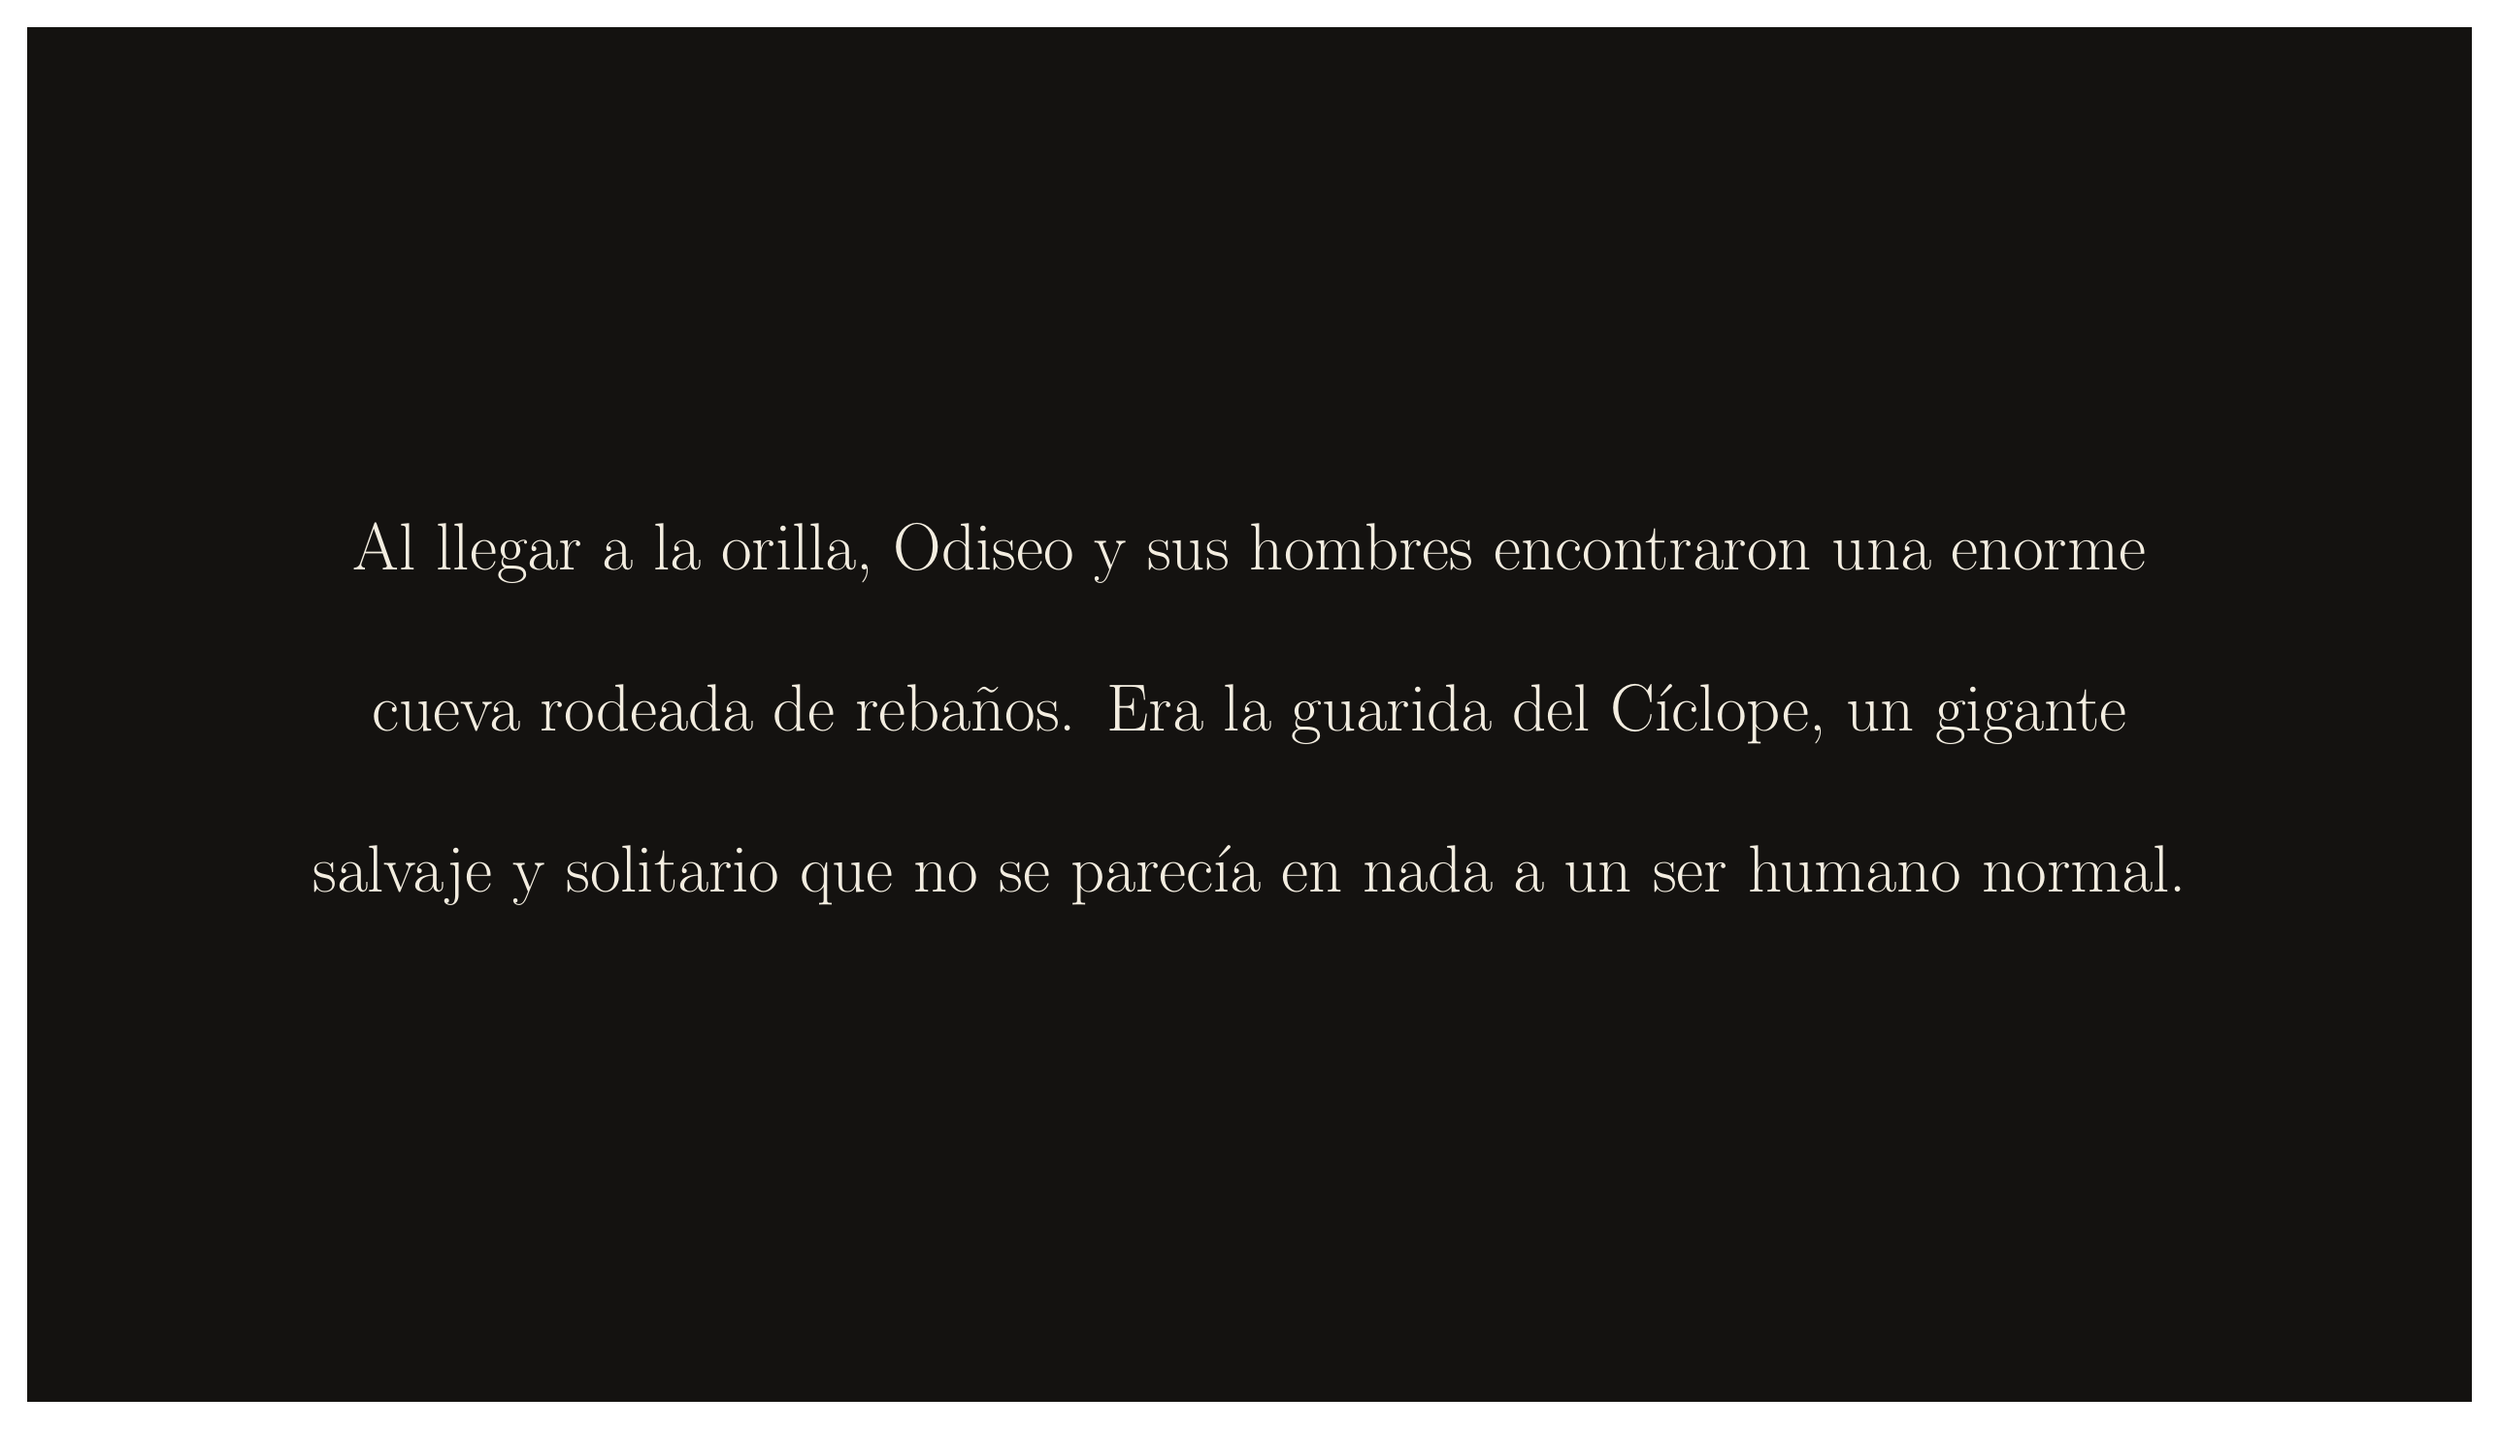
\begin{tikzpicture}
  % Área fija 16:9
  \useasboundingbox (0,0) rectangle (\ancho,\alto);
  \fill[Fondo] (0,0) rectangle (\ancho,\alto);

  % Texto procesado
  \node[text=Texto, align=center, text width=\AnchoTexto cm,
        font=\fontsize{\TamLetra}{\Interlinea}\selectfont]
    at (\ancho/2,\alto/2) {%
      Al llegar a la orilla, Odiseo y sus hombres encontraron una enorme
      cueva rodeada de rebaños. Era la guarida del Cíclope, un gigante
      salvaje y solitario que no se parecía en nada a un ser humano normal.%
    };
\end{tikzpicture}
\end{document}
